% Submission draft formatted for EMNLP 2026 with the official ACL style files.
% Review mode; all quantitative claims are macros generated by paper/gen_paper.py.
\documentclass[11pt]{article}
\usepackage[review]{acl}
\usepackage{times}
\usepackage{latexsym}
\usepackage[T1]{fontenc}
\usepackage[utf8]{inputenc}
\usepackage{microtype}
\usepackage{graphicx}
\usepackage{booktabs}
\usepackage{amsmath,amssymb}
\usepackage{url}
\usepackage{inconsolata}

\graphicspath{{generated/}}
\setlength{\emergencystretch}{2em}

\title{\textbf{More Context, Less Accuracy:}\\[0.2em]
A Pre-Registered Negative Result for a Byte-Level Decider}

\author{}

\begin{document}
\maketitle

% generated by paper/gen_paper.py -- do not edit by hand
\newcommand{\PJevAcc}{92.40}
\newcommand{\PJevCorrect}{2{,}846}
\newcommand{\PN}{3{,}080}
\newcommand{\PLabels}{77}
\newcommand{\PExamples}{24}
\newcommand{\PBar}{92.40}
\newcommand{\PMargin}{2.0}
\newcommand{\PNativeBudget}{1{,}020}
\newcommand{\PLongBudget}{5{,}118}
\newcommand{\POldZeroAcc}{88.38}
\newcommand{\POldZeroLo}{87.20}
\newcommand{\POldZeroHi}{89.46}
\newcommand{\POldZeroCorrect}{2{,}722}
\newcommand{\POldZeroN}{3{,}080}
\newcommand{\POldZeroExamples}{0.0}
\newcommand{\POldZeroExamplesMin}{0}
\newcommand{\POldZeroExamplesMax}{0}
\newcommand{\POldZeroContext}{54}
\newcommand{\POldZeroGap}{$-4.03$}
\newcommand{\POldZeroLower}{$-4.97$}
\newcommand{\POldZeroP}{$8.49\times10^{-12}$}
\newcommand{\POldZeroPText}{$p = 8.49\times10^{-12}$}
\newcommand{\POldTwoAcc}{59.12}
\newcommand{\POldTwoLo}{57.38}
\newcommand{\POldTwoHi}{60.85}
\newcommand{\POldTwoCorrect}{1{,}821}
\newcommand{\POldTwoN}{3{,}080}
\newcommand{\POldTwoExamples}{11.9}
\newcommand{\POldTwoExamplesMin}{2}
\newcommand{\POldTwoExamplesMax}{19}
\newcommand{\POldTwoContext}{978}
\newcommand{\POldTwoGap}{$-33.28$}
\newcommand{\POldTwoLower}{$-34.87$}
\newcommand{\POldTwoP}{$2.96\times10^{-231}$}
\newcommand{\POldTwoPText}{$p = 2.96\times10^{-231}$}
\newcommand{\POldLenAcc}{22.44}
\newcommand{\POldLenLo}{21.00}
\newcommand{\POldLenHi}{23.94}
\newcommand{\POldLenCorrect}{691}
\newcommand{\POldLenN}{3{,}080}
\newcommand{\POldLenExamples}{24.0}
\newcommand{\POldLenExamplesMin}{24}
\newcommand{\POldLenExamplesMax}{24}
\newcommand{\POldLenContext}{1{,}987}
\newcommand{\POldLenGap}{$-69.97$}
\newcommand{\POldLenLower}{$-71.40$}
\newcommand{\POldLenP}{$<10^{-300}$}
\newcommand{\POldLenPText}{$p<10^{-300}$}
\newcommand{\PQueryZeroAcc}{61.04}
\newcommand{\PQueryZeroLo}{59.30}
\newcommand{\PQueryZeroHi}{62.75}
\newcommand{\PQueryZeroCorrect}{1{,}880}
\newcommand{\PQueryZeroN}{3{,}080}
\newcommand{\PQueryZeroExamples}{0.0}
\newcommand{\PQueryZeroExamplesMin}{0}
\newcommand{\PQueryZeroExamplesMax}{0}
\newcommand{\PQueryZeroContext}{54}
\newcommand{\PQueryZeroGap}{$-31.36$}
\newcommand{\PQueryZeroLower}{$-32.82$}
\newcommand{\PQueryZeroP}{$1.82\times10^{-226}$}
\newcommand{\PQueryZeroPText}{$p = 1.82\times10^{-226}$}
\newcommand{\PQueryTwoAcc}{89.03}
\newcommand{\PQueryTwoLo}{87.87}
\newcommand{\PQueryTwoHi}{90.08}
\newcommand{\PQueryTwoCorrect}{2{,}742}
\newcommand{\PQueryTwoN}{3{,}080}
\newcommand{\PQueryTwoExamples}{11.9}
\newcommand{\PQueryTwoExamplesMin}{2}
\newcommand{\PQueryTwoExamplesMax}{19}
\newcommand{\PQueryTwoContext}{978}
\newcommand{\PQueryTwoGap}{$-3.38$}
\newcommand{\PQueryTwoLower}{$-4.32$}
\newcommand{\PQueryTwoP}{$3.99\times10^{-9}$}
\newcommand{\PQueryTwoPText}{$p = 3.99\times10^{-9}$}
\newcommand{\PLenZeroAcc}{61.75}
\newcommand{\PLenZeroLo}{60.02}
\newcommand{\PLenZeroHi}{63.45}
\newcommand{\PLenZeroCorrect}{1{,}902}
\newcommand{\PLenZeroN}{3{,}080}
\newcommand{\PLenZeroExamples}{0.0}
\newcommand{\PLenZeroExamplesMin}{0}
\newcommand{\PLenZeroExamplesMax}{0}
\newcommand{\PLenZeroContext}{54}
\newcommand{\PLenZeroGap}{$-30.65$}
\newcommand{\PLenZeroLower}{$-32.11$}
\newcommand{\PLenZeroP}{$1.62\times10^{-232}$}
\newcommand{\PLenZeroPText}{$p = 1.62\times10^{-232}$}
\newcommand{\PLenTwoAcc}{87.11}
\newcommand{\PLenTwoLo}{85.88}
\newcommand{\PLenTwoHi}{88.25}
\newcommand{\PLenTwoCorrect}{2{,}683}
\newcommand{\PLenTwoN}{3{,}080}
\newcommand{\PLenTwoExamples}{24.0}
\newcommand{\PLenTwoExamplesMin}{24}
\newcommand{\PLenTwoExamplesMax}{24}
\newcommand{\PLenTwoContext}{1{,}988}
\newcommand{\PLenTwoGap}{$-5.29$}
\newcommand{\PLenTwoLower}{$-6.30$}
\newcommand{\PLenTwoP}{$5.01\times10^{-18}$}
\newcommand{\PLenTwoPText}{$p = 5.01\times10^{-18}$}
\newcommand{\PQueryGap}{$-3.38$}
\newcommand{\PQueryGapAbs}{3.38}
\newcommand{\PQueryLower}{$-4.32$}
\newcommand{\PQueryP}{$3.99\times10^{-9}$}
\newcommand{\PQueryPText}{$p = 3.99\times10^{-9}$}
\newcommand{\PQueryNonInf}{no}
\newcommand{\PLenGap}{$-5.29$}
\newcommand{\PLenGapAbs}{5.29}
\newcommand{\PLenTwoGapAbs}{5.29}
\newcommand{\PLenLower}{$-6.30$}
\newcommand{\PLenP}{$5.01\times10^{-18}$}
\newcommand{\PLenPText}{$p = 5.01\times10^{-18}$}
\newcommand{\PLenNonInf}{no}
\newcommand{\PMechGain}{+29.90}
\newcommand{\PMechGainAbs}{29.90}
\newcommand{\PMechLower}{+28.41}
\newcommand{\PMechP}{$3.62\times10^{-212}$}
\newcommand{\PMechPText}{$p = 3.62\times10^{-212}$}
\newcommand{\PLenMechGain}{+27.99}
\newcommand{\PLenMechLower}{+26.46}
\newcommand{\PLenMechP}{$6.90\times10^{-180}$}
\newcommand{\PQueryVsOldZero}{+0.65}
\newcommand{\PQueryVsOldZeroLower}{$-0.26$}
\newcommand{\PQueryVsOldZeroP}{$2.60\times10^{-1}$}
\newcommand{\PQueryVsOldZeroPText}{$p = 2.60\times10^{-1}$}
\newcommand{\POldVsMessage}{$-29.25$}
\newcommand{\POldVsMessageLower}{$-30.81$}
\newcommand{\POldVsMessageP}{$4.23\times10^{-188}$}
\newcommand{\POldVsMessagePText}{$p = 4.23\times10^{-188}$}
\newcommand{\PLenVsNative}{$-1.92$}
\newcommand{\PLenVsNativeLower}{$-2.69$}
\newcommand{\PLenVsNativeP}{$8.75\times10^{-5}$}
\newcommand{\PLenVsNativePText}{$p = 8.75\times10^{-5}$}
\newcommand{\PLenVsOldZero}{$-1.27$}
\newcommand{\PLenVsOldZeroLower}{$-2.27$}
\newcommand{\PLenVsOldZeroP}{$3.83\times10^{-2}$}
\newcommand{\PLenVsOldZeroPText}{$p = 3.83\times10^{-2}$}
\newcommand{\PLenVsOldTwo}{+27.99}
\newcommand{\PLenVsOldTwoLower}{+26.46}
\newcommand{\PLenVsOldTwoP}{$6.90\times10^{-180}$}
\newcommand{\PLenVsLenZero}{+25.36}
\newcommand{\PLenVsLenZeroLower}{+23.93}
\newcommand{\PLenVsLenZeroP}{$1.27\times10^{-173}$}
\newcommand{\PQueryEff}{11.9}
\newcommand{\PQueryEffMin}{2}
\newcommand{\PQueryEffMax}{19}
\newcommand{\PLenEff}{24.0}
\newcommand{\PLenEffMin}{24}
\newcommand{\PLenEffMax}{24}
\newcommand{\PJevDefsBytes}{7{,}801}
\newcommand{\PJevQuestionBytes}{8{,}187}
\newcommand{\PJevPromptMedian}{10{,}683}
\newcommand{\PJevPromptMin}{10{,}009}
\newcommand{\PJevPromptMax}{13{,}524}
\newcommand{\PJevPromptMean}{10{,}783}
\newcommand{\PJevExamplesMedian}{2{,}367}
\newcommand{\PJevPromptRatio}{2.09}
\newcommand{\PJevPromptMaxRatio}{2.64}
\newcommand{\PJevDefsRatio}{1.52}
\newcommand{\PAzuriteShare}{47.9}
\newcommand{\PJevDefsShare}{73.0}
\newcommand{\PContamSupportRows}{9{,}993}
\newcommand{\PContamSupportClean}{9{,}968}
\newcommand{\PContamSupportMatches}{25}
\newcommand{\PContamSupportExact}{6}
\newcommand{\PContamSupportShare}{0.25}
\newcommand{\PContamSupportSameLabel}{25}
\newcommand{\PContamEvalRows}{255}
\newcommand{\PContamEvalShare}{8.28}
\newcommand{\PContamInstances}{283}
\newcommand{\PContamSelf}{25}
\newcommand{\PContamCross}{258}
\newcommand{\PContamCrossRows}{236}
\newcommand{\PContamCrossOnly}{230}
\newcommand{\PContamSameLabel}{81}
\newcommand{\PContamDiffLabel}{202}
\newcommand{\PContamExactExamples}{6}
\newcommand{\PContamUnique}{25}
\newcommand{\PCleanN}{3{,}080}
\newcommand{\PCleanCorrect}{2{,}743}
\newcommand{\PCleanAcc}{89.06}
\newcommand{\PCleanLo}{87.91}
\newcommand{\PCleanHi}{90.11}
\newcommand{\PCleanDiff}{+0.03}
\newcommand{\PCleanDiffAbs}{0.03}
\newcommand{\PCleanWins}{2}
\newcommand{\PCleanLosses}{1}
\newcommand{\PCleanP}{1.00}
\newcommand{\PCleanPText}{p = 1.00}
\newcommand{\PUnaffectedN}{2{,}825}
\newcommand{\PUnaffectedCorrect}{2{,}511}
\newcommand{\PUnaffectedAcc}{88.88}
\newcommand{\PUnaffectedLo}{87.67}
\newcommand{\PUnaffectedHi}{89.99}
\newcommand{\PContamContextChanged}{256}
\newcommand{\PContamPredSame}{3{,}077}
\newcommand{\PContamProductFrozenSameContext}{2{,}971}
\newcommand{\PContamProductFrozenDiscordant}{0}
\newcommand{\PParams}{113{,}465{,}856}
\newcommand{\PParamsM}{113.47}
\newcommand{\PNativeSeq}{1{,}024}
\newcommand{\PBOOT}{10{,}000}
\newcommand{\PTrainN}{4{,}000}
\newcommand{\PTrainCorrect}{3{,}865}
\newcommand{\PSteps}{3{,}000}
\newcommand{\PBatch}{8}
\newcommand{\PSeq}{5{,}120}
\newcommand{\PTokens}{122{,}880{,}000}
\newcommand{\PGPUHours}{1.69}
\newcommand{\PSecStep}{2.02}
\newcommand{\PTrainAcc}{96.62}
\newcommand{\PTestAcc}{87.11}
\newcommand{\PTrainGap}{$-9.51$}
\newcommand{\PTrainLoss}{0.1321}
\newcommand{\PLastLoss}{0.7271}
\newcommand{\PMeanLastFifty}{0.2214}
\newcommand{\PQueryPrereg}{bde97e74f2f8}
\newcommand{\PLenPrereg}{c59b5e08d916}
\newcommand{\PLenAmendment}{7993177d769a}
\newcommand{\PInputs}{8dccd8c89886}
\newcommand{\POldHead}{42f1ed1c8471}
\newcommand{\PQueryHead}{7992c97362b3}
\newcommand{\PLenHead}{e7455fc462e9}
\newcommand{\PLenInit}{5294fd685615}
\newcommand{\PCodeQuery}{95a5e0a5d11e}
\newcommand{\PCodeLen}{0800b2aad102}
\newcommand{\PQueryVerdict}{P0 missed}
\newcommand{\PLenVerdict}{P0 missed}
\newcommand{\PJevMismatchGap}{$-69.97$}
\newcommand{\POldZeroDistinct}{77}
\newcommand{\POldZeroTop}{1.62}
\newcommand{\POldZeroTopThree}{4.77}
\newcommand{\POldTwoDistinct}{77}
\newcommand{\POldTwoTop}{3.80}
\newcommand{\POldTwoTopThree}{10.19}
\newcommand{\POldLenDistinct}{64}
\newcommand{\POldLenTop}{14.29}
\newcommand{\POldLenTopThree}{35.36}
\newcommand{\PQueryZeroDistinct}{77}
\newcommand{\PQueryZeroTop}{4.12}
\newcommand{\PQueryZeroTopThree}{11.33}
\newcommand{\PQueryTwoDistinct}{77}
\newcommand{\PQueryTwoTop}{1.59}
\newcommand{\PQueryTwoTopThree}{4.64}
\newcommand{\PLenZeroDistinct}{77}
\newcommand{\PLenZeroTop}{2.60}
\newcommand{\PLenZeroTopThree}{7.79}
\newcommand{\PLenTwoDistinct}{77}
\newcommand{\PLenTwoTop}{1.69}
\newcommand{\PLenTwoTopThree}{4.94}


\begin{abstract}
A decider replaces generation with scoring a finite candidate set. The
architectural promise is that a small local model can match a hosted service at
a fraction of the cost, but the promise is usually tested on a different row
set, a different prompt and a different notion of ``the same information''. We
run the comparison the promise needs. On all \PN{} official Banking77 test
rows, with the exact \PExamples{} retrieved examples and the frozen per-row
correctness vector of a \PJevAcc\% Jev run, a \PParamsM{}M-parameter byte-level
decider reaches \PQueryTwoAcc\% (95\% Wilson \PQueryTwoLo--\PQueryTwoHi), a gap
of \PQueryGapAbs{} points. The pre-registered bar is missed (exact McNemar
\PQueryPText; paired 95\% lower bound \PQueryLower{} points). The frozen
examples contain \PContamSupportMatches{} test messages (\PContamEvalRows{} rows
retrieve at least one); a decontaminated rerun scores \PCleanAcc\%, so the gap
is not an artefact of that overlap.

The negative result has a located mechanism. Mean pooling dilutes the customer
message into the retrieved examples: the same encoder falls from
\POldZeroAcc\% message-only to \POldTwoAcc\% with examples at its native
\PNativeBudget-byte window, and to \POldLenAcc\% when all \PExamples{} examples
are packed at \PSeq{} bytes. Replacing mean pooling with a message-query
attention pool recovers \PMechGain{} points on identical contexts
(\PMechLower{} lower bound), which identifies the pooling operation rather than
the examples as the immediate cause. The fix is real but not sufficient. The
query head with examples is only \PQueryVsOldZero{} points above the old head's
message-only arm (not significant; \PQueryVsOldZeroPText), and a joint
\PSeq-byte fine-tune that fits all \PExamples{} examples reaches \PLenTwoAcc\%,
below both the native-window query head and the message-only head.

The comparator's reconstructed JSON prompt is \PJevPromptMedian{} bytes in the
median, \PJevPromptRatio$\times$ the largest context we test, and contains the
\PLabels{} category definitions that no Azurite arm receives. The comparison is therefore not information-matched. We publish the full per-row records, the
hashes and a generator that recomputes every number in this paper.
\end{abstract}

\section{Introduction}

A decider constrains a model's output to a declared candidate set.\footnote{This
manuscript is formatted for EMNLP 2026 using the official ACL style files in
review mode.} Instead of generating a label token by token, it scores every
candidate and returns the argmax; an out-of-bank answer is impossible by
construction. TypeSafe's Jev
markets this interface as a ``System One'' model: all outputs are generated in a
single query, the possible outputs are defined in advance, and the service is
priced per input token \citep{typesafe2026jev}. The interface is attractive for
classification, routing and extraction because it converts an open-ended
generation problem into a finite comparison.

The commercial argument is comparative: a compact local decider should be
faster, smaller and cheaper than a hosted decider at equal accuracy. The
accuracy clause is the hard one. A hosted decider can be given a long prompt
with category definitions and retrieved labelled examples; a local decider is
limited by its context window, its training distribution and its pooling
operation. If the local model fails, the failure could be the architecture, the
information, or the interface. A comparison that changes all three at once
cannot say which.

This paper isolates one of those changes. We take a frozen third-party run of
Jev 1.13 on the complete official Banking77 test set: \PJevCorrect{} of \PN{}
rows correct (\PJevAcc\%), with the exact \PExamples{} BM25-retrieved labelled
examples and all \PLabels{} category definitions supplied for every row
\citep{smith2026jevbanking}. We give Azurite, a \PParamsM{}M-parameter
byte-level encoder with a decider head, the same rows, the same gold labels,
the same \PExamples{} examples and the same frozen Jev correctness vector. We
withhold the category definitions, so Azurite's information budget is strictly
smaller; that asymmetry is stated before the result and favours Jev. We then
vary the head and the context budget under separate pre-registrations.

The headline is negative. The best arm reaches \PQueryTwoAcc\%, \PQueryGapAbs{}
points below Jev, and the pre-registered P0 rule is missed. We report that
plainly. The more useful result is why. Mean pooling, which is the default for
sentence-level classification, averages every non-padding token. A context with
a short customer message and several retrieved examples is mostly examples, so
the pooled vector stops being a representation of the message. The same encoder
therefore loses \POldTwoGap{} points when examples are added at its native
window, and collapses to \POldLenAcc\% when all \PExamples{} examples are packed
at \PSeq{} bytes. A message-query attention pool removes that dilution and
recovers \PMechGain{} points on identical contexts. That is a clean mechanism
result: the examples were readable, but the read-out was averaging them away.

Removing the pooling bottleneck does not recover the accuracy. The query head
with examples is statistically indistinguishable from the old head with no
examples at all (\PQueryVsOldZero{} points, \PQueryVsOldZeroPText). Extending
the context to \PSeq{} bytes so that all \PExamples{} examples fit makes things
worse: the joint fine-tune reaches \PLenTwoAcc\%, \PLenVsNative{} points below
the native query head and \PLenVsOldZero{} points below the old message-only
head. The example budget is not the missing variable. The comparator's
reconstructed JSON prompt is \PJevPromptMedian{} bytes in the median and
\PJevDefsBytes{} of those bytes are the \PLabels{} definitions; our largest
context is \PAzuriteShare\% of the median prompt and contains no definitions.
The experiment therefore bounds the claim it can make. It shows that this
decoder, with this information budget and this pooling, cannot reach the bar.
It does not show that a decider with information parity cannot.

\paragraph{Contributions.}
\begin{enumerate}
  \item A pre-registered comparison on the full \PN-row Banking77 test set,
  using the exact per-row examples and frozen correctness vector of a public
  \PJevAcc\% Jev run, with paired Wilson, McNemar and bootstrap inference.
  \item A located mechanism for the failure: mean-pool dilution, isolated by a
  same-context head control and a message-only control, and corroborated by
  prediction concentration on the stored per-row predictions.
  \item A bound on the example-budget explanation: all \PExamples{} examples fit
  at \PSeq{} bytes, yet accuracy falls; the comparator prompt is
  \PJevPromptRatio$\times$ larger and includes definitions. The remaining gap is
  an information-and-scale question, not another head.
  \item A reproducibility artifact: every number, table and figure is emitted
  from the stored summaries by one generator, with a reconciliation record that
  also checks the overlapping thesis values.
\end{enumerate}

\paragraph{Scope.}
This is a study of a text-only, byte-level decider at a \PSeq-byte context. It
makes no claim about multimodal models or about long-context models in the
modern sense: \PSeq{} bytes is four times the native window but orders of
magnitude below the contexts used in long-context evaluations
\citep{liu2023lost,hsieh2024ruler}. The negative result is correspondingly
narrow, and we state the boundary explicitly rather than extrapolating from it.

\section{Related Work}

\paragraph{Deciders and constrained output.}
Jev is the closest comparator: a hosted service that returns one of a declared
set of outputs and reports per-token pricing and latency
\citep{typesafe2026jev}. The public Banking77 run we use supplies retrieved
examples and category definitions and scores all \PN{} test rows
\citep{smith2026jevbanking}. Constrained decoding and candidate scoring are
older ideas; what is new in the decider framing is the claim that a finite,
declared output space makes a small model competitive with open-ended
generation. Our experiment tests the accuracy half of that claim under a
matched row set, not the pricing half.

\paragraph{Retrieval and in-context examples.}
Retrieval-augmented models condition on passages or demonstrations selected at
inference time \citep{karpukhin2020dpr,lewis2020rag}. Few-shot prompting shows
that demonstrations can change a model's behaviour substantially
\citep{brown2020gpt3}, but the effect is not simply ``more examples, more
accuracy'': demonstrations can supply the label space and the format while the
input-label mapping matters less than expected \citep{min2022rethinking}, and
many-shot regimes can behave differently from few-shot ones
\citep{agarwal2024manyshot}. Our result is consistent with that literature but
is a different failure: the examples are not ignored, they are averaged into
the representation until the message is no longer recoverable.

\paragraph{Byte-level encoders.}
Byte-level models remove the tokeniser and make the input distribution uniform
over bytes \citep{xue2022byt5,clark2022canine}. That is attractive for a decider
because the candidate set and the input share one alphabet, and because
arbitrary labels can be scored without a tokenisation mismatch. The cost is a
longer sequence for the same text and a greater sensitivity to context length.
Azurite is a masked byte-level encoder in this line; the head is a candidate
scorer rather than a generator.

\paragraph{Evaluation and inference.}
A single accuracy on a single draw is a noisy estimate. We use Wilson score
intervals \citep{wilson1927}, exact McNemar tests on paired correctness
\citep{mcnemar1947} and a paired bootstrap lower bound, following the
recommendation that classifier comparisons be paired rather than treated as
independent samples \citep{dietterich1998}. The protocols were written and
hashed before evaluation; amendments are recorded and limited to evaluator or
schedule changes. This is a small methodological contribution, but it is what
makes a negative result interpretable.

\section{Protocol}
\label{sec:protocol}

\subsection{Task and frozen comparator}

Banking77 is a fine-grained intent classification task with \PLabels{} banking
intents \citep{casanueva2020banking}. We use the official test split of \PN{}
rows and the \PTrainN{} training rows. The public Jev run supplies, for every
test row, the customer message, the gold label, the Jev prediction, a binary
Jev-correctness bit, and exactly \PExamples{} BM25-retrieved labelled training
examples with all \PLabels{} category definitions \citep{smith2026jevbanking}.
We freeze that record before any Azurite forward pass: the row order, the
examples, the gold labels and the Jev correctness vector are identical in every
arm. The frozen vector has \PJevCorrect{} correct rows, so the pre-registered
P0 bar is \PBar\%.

BM25 is the retriever used by the public harness
\citep{robertson2009bm25}. The retrieval is not re-run: we take the stored
example ids and messages exactly as the public run recorded them. The public
run describes the examples as training-split retrievals, but the stored record
does not fully support that description. Under normalised text (NFKC,
case-folding, punctuation collapsed), \PContamSupportMatches{} of the
\PContamSupportRows{} support messages are official test rows
(\PContamSupportExact{} exact; \PContamSupportShare\% of the bank), and all
carry the same gold label. They occur in the frozen example sets of
\PContamEvalRows{} of the \PN{} rows (\PContamEvalShare\%), as
\PContamInstances{} instances: \PContamSelf{} self-retrievals and
\PContamCross{} cross-row retrievals. The contamination is not uniform:
\PUnaffectedN{} rows retrieve no test text. The frozen set therefore contradicts
the comparator's description of its examples as training-split-only retrievals.

The original product path over the \PContamSupportRows{}-row bank is not an
independent corroboration: it produced the same prediction on all \PN{} rows and
the same context digest on \PContamProductFrozenSameContext{} of them. Removing
all \PContamSupportMatches{} test messages from the support bank and re-running
gives \PCleanAcc\%
(\PCleanCorrect/\PCleanN; 95\% Wilson \PCleanLo--\PCleanHi), a change of
\PCleanDiff{} points (\PCleanWins{} wins, \PCleanLosses{} loss; exact McNemar
\PCleanPText). The \PUnaffectedN{} unaffected rows score \PUnaffectedAcc\%
(\PUnaffectedCorrect/\PUnaffectedN; 95\% Wilson \PUnaffectedLo--\PUnaffectedHi).
The overlap does not explain the gap, but \PQueryTwoAcc\% is not a clean
held-out estimate and must not be presented as one.

\subsection{Model and arms}

Azurite is a \PParamsM{}M-parameter masked byte-level encoder
\citep{xue2022byt5,clark2022canine}, built from transformer blocks
\citep{vaswani2017attention} and trained with a masked objective
\citep{devlin2019bert}. The encoder has a native window of
\PNativeSeq{} bytes. Two heads are compared.

\paragraph{Old head.} A mean-pool over every non-padding token, followed by a
linear projection to the \PLabels{} candidate embeddings. This is the standard
sentence-classification read-out and the head used by the earlier suite. It is
trained on \PTrainN{} rows with the message only.

\paragraph{Query head.} A masked attention pool whose query is a linear map of
the mean-pooled customer message. Candidate embeddings are shared with the old
head's projection. The head is trained on the same \PTrainN{} rows, but the
contexts contain retrieved examples; the message-query is what keeps the
message from being averaged away.

Table~\ref{tab:main} lists the arms. The old head is evaluated at
\PNativeBudget{} bytes (message only and the examples that fit) and at
\PSeq{} bytes with all \PExamples{} examples. The query head is evaluated at
\PNativeBudget{} bytes (message only and examples) and at \PSeq{} bytes with
all \PExamples{} examples. The \PSeq{}-byte query arm is a joint fine-tune: the
encoder and head are trained together for \PSteps{} steps at batch \PBatch{},
which is \PTokens{} byte positions and \PGPUHours{} GPU-hours on one RTX PRO
6000. The original two-stage length-adaptation schedule was replaced by this
joint schedule in a hashed amendment before any \PSeq-byte accuracy existed;
the amendment changes the schedule, not the question, rows, examples or
decision rule. The joint schedule means the arm cannot separate length from
head training, and we treat it that way.

\paragraph{Decision rule.}\label{sec:decision} The primary arm is fixed in advance. The P0 bar is
Jev's point estimate, \PBar\%. The arm \emph{exceeds} P0 if its point estimate
is above the bar and the exact two-sided McNemar test against the frozen Jev
vector has $p<0.05$. It \emph{meets} P0 if its point estimate is at least the
bar. It \emph{misses} P0 otherwise. Non-inferiority is reported separately: the
5th percentile of \PBOOT{} paired bootstrap resamples (seed 0) must exceed
$-\PMargin$ points. No early stopping, checkpoint selection or best-of-steps choice
is used; the final step is evaluated.

\begin{table*}[t]
\centering
\footnotesize
\caption{The pre-registered comparison on all \PN{} official Banking77 test rows.
\emph{Old} is the mean-pool head; \emph{query} is the message-query attention
head. The byte budget names the context window; \emph{examples} is the mean
number of complete retrieved examples that fit (range in the text). The
old-head 5{,}120 arm is the matched-test packing of all 24 examples; its native
control is the query-evaluation packing, which averages \POldTwoExamples{}
examples. The Jev row is the cited public run, not a rerun; its Bytes cell is
the reconstructed JSON prompt size, not a model context window. Wilson
intervals are 95\%; $\Delta$ and exact two-sided McNemar $p$ are against Jev's frozen
per-row correctness vector. The 5{,}120 query head is a joint encoder/head
fine-tune, not a length-only adaptation. Every cell is generated from
\texttt{results/jev\_query}, \texttt{results/jev\_query\_5120} or
\texttt{results/jev\_matched}.}
\label{tab:main}
\setlength{\tabcolsep}{3pt}
\begin{tabular}{@{}lrrrrrrrr@{}}
\toprule
Arm & Ex. & Bytes & $n$ & Correct & Acc. & 95\% Wilson & $\Delta$ vs Jev & McNemar $p$ \\
 & & & & & (\%) & & (pp) & \\
\midrule
Old mean-pool, message only & 0.0 & 54 & 3{,}080 & 2{,}722 & 88.38 & 87.20--89.46 & $-4.03$ & $8.49\times10^{-12}$ \\
Old mean-pool, examples that fit & 11.9 & 978 & 3{,}080 & 1{,}821 & 59.12 & 57.38--60.85 & $-33.28$ & $2.96\times10^{-231}$ \\
Old mean-pool, all 24 at 5{,}120 & 24.0 & 1{,}987 & 3{,}080 & 691 & 22.44 & 21.00--23.94 & $-69.97$ & $<10^{-300}$ \\
Query attention, message only & 0.0 & 54 & 3{,}080 & 1{,}880 & 61.04 & 59.30--62.75 & $-31.36$ & $1.82\times10^{-226}$ \\
Query attention, examples that fit & 11.9 & 978 & 3{,}080 & 2{,}742 & 89.03 & 87.87--90.08 & $-3.38$ & $3.99\times10^{-9}$ \\
Query attention, 5{,}120, message only & 0.0 & 54 & 3{,}080 & 1{,}902 & 61.75 & 60.02--63.45 & $-30.65$ & $1.62\times10^{-232}$ \\
Query attention, 5{,}120, all 24 & 24.0 & 1{,}988 & 3{,}080 & 2{,}683 & 87.11 & 85.88--88.25 & $-5.29$ & $5.01\times10^{-18}$ \\
Jev 1.13, cited & 24 & 10{,}683 & 3{,}080 & 2{,}846 & 92.40 & 91.41--93.29 & --- & --- \\
\bottomrule
\end{tabular}
\end{table*}


\subsection{Provenance}

The query protocol is hashed as \texttt{\PQueryPrereg}; the \PSeq-byte
protocol as \texttt{\PLenPrereg} and its schedule amendment as
\texttt{\PLenAmendment}. The frozen inputs hash to \texttt{\PInputs}; the old
head to \texttt{\POldHead}, the query head to \texttt{\PQueryHead}, and the
\PSeq-byte head to \texttt{\PLenHead}. The \PSeq-byte run starts from the
\PNativeSeq-position checkpoint \texttt{\PLenInit}. Table~\ref{tab:hashes} in
the appendix lists the same values, and \texttt{paper/RECONCILIATION.md}
records where each paper number comes from.

Every arm writes one JSONL record per row with the row id, the gold index, the
predicted index, the correctness bit, the context hash, the context byte count
and the number of effective examples. The evaluation summary is generated from
those files, not typed. The generator verifies each file's SHA-256, recomputes
every accuracy and Wilson interval, reruns every McNemar test and bootstrap
from the aligned vectors, and refuses to write a macro if a stored value
differs.

\subsection{The information budget}

The comparison is only interpretable if we know how much information each
system receives. Azurite's largest context is \PLongBudget{} bytes: all
\PExamples{} examples fit, but the \PLabels{} definitions do not. The public Jev
harness serializes a JSON payload with the message, the labelled examples and
the \PLabels{} definitions in a single choice question. We reconstruct that
payload from the harness's published description and category files and the
stored per-row examples, using the harness's own instruction string. The
definitions alone are \PJevDefsBytes{} bytes; the full payload has a median of
\PJevPromptMedian{} bytes (range \PJevPromptMin--\PJevPromptMax), of which
\PJevExamplesMedian{} bytes are the retrieved examples. Azurite's \PLongBudget{}
bytes are \PAzuriteShare\% of that median. The reconstruction is not an invoice
and does not recover the exact serialized prompt Jev received; it establishes
the order of magnitude and the presence of the definitions, which is all the
argument needs.

\section{Results}

\subsection{The pre-registered comparison}

The primary arm reaches \PQueryTwoAcc\% (95\% Wilson
\PQueryTwoLo--\PQueryTwoHi; \PQueryTwoCorrect/\PN). Jev's frozen vector is
\PJevAcc\% (\PJevCorrect/\PN). The observed difference is \PQueryGap{} points;
the exact McNemar test gives \PQueryPText; the paired bootstrap lower bound is
\PQueryLower{} points. The arm is not non-inferior at the $-\PMargin$-point margin
(non-inferiority: \PQueryNonInf), and the pre-registered verdict is \textbf{\PQueryVerdict}. The
interval does not contain the bar.

This is the result the paper is about, and it is a loss. The contamination audit
in \S\ref{sec:protocol} changes its interpretation, not its verdict: the frozen
\PQueryTwoAcc\% includes \PContamEvalRows{} rows that retrieve test text, while
the decontaminated rerun scores \PCleanAcc\% and the unaffected rows
\PUnaffectedAcc\%. The loss is not an artefact of the overlap, but the frozen
number is not clean. The remaining sections ask why, and which part of the loss
is a head problem rather than an information problem.

\subsection{Mean pooling is the immediate cause}

The old head gives a clean dose-response curve at its native window. With the
message only it reaches \POldZeroAcc\% (\POldZeroLo--\POldZeroHi). With the
examples that fit in \PNativeBudget{} bytes---\PQueryEff{} on average, range
\PQueryEffMin--\PQueryEffMax---it falls to \POldTwoAcc\%
(\POldTwoLo--\POldTwoHi), a loss of \POldTwoGap{} points. At \PSeq{} bytes with
all \PExamples{} examples it reaches \POldLenAcc\% (\POldLenLo--\POldLenHi),
\POldLenGap{} points below Jev. The last arm changes both examples and length,
so it is not a clean examples-only manipulation; the native-window arm is. Even
there, the examples-only change is \POldVsMessage{} points (exact McNemar
\POldVsMessagePText).

The query head isolates the read-out. On the identical \PNativeBudget-byte
contexts, it reaches \PQueryTwoAcc\% against the old head's \POldTwoAcc\%, a
gain of \PMechGain{} points (exact McNemar \PMechPText; bootstrap lower
\PMechLower). The only difference between those two arms is the pooling
operation and the head trained with it; the rows, the examples, the encoder
initialisation, the training rows and the evaluation rows are the same. The
pooling diagnosis is therefore confirmed at the level of the head: the examples
were not unreadable, they were being averaged away.

The prediction concentration tells the same story from the output side
(Figure~\ref{fig:concentration}). The old head at \PSeq{} bytes uses
\POldLenDistinct{} of the \PLabels{} labels; its most frequent label takes
\POldLenTop\% of rows and its three most frequent take \POldLenTopThree\%.
The message-only old head uses all \PLabels{} labels with a top-1 share of
\POldZeroTop\% and a top-3 share of \POldZeroTopThree\%. The query head with
examples returns to \PQueryTwoTop\% and \PQueryTwoTopThree\% with all
\PLabels{} labels. The old head is not failing because it cannot represent the
labels; it is failing because the pooled context drifts toward whichever
intents dominate the retrieved examples.

\begin{figure}[t]
\centering
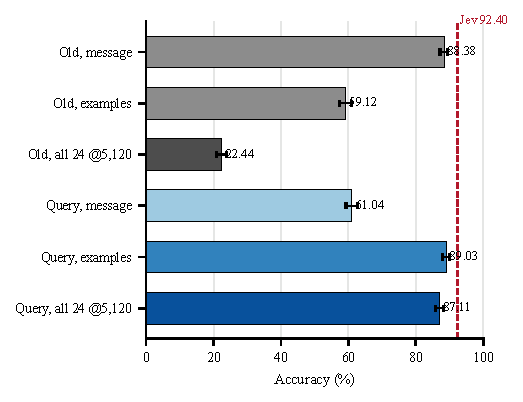
\includegraphics[width=\linewidth]{fig_accuracy.pdf}
\caption{Accuracy on all \PN{} official Banking77 rows with 95\% Wilson
intervals. The dashed line is Jev's frozen \PJevAcc\%. The old head loses
accuracy monotonically as examples are added; the query head recovers the
native-window loss but does not beat the message-only old head. The
\PSeq-byte query arm is a joint fine-tune, not a length-only adaptation.}
\label{fig:accuracy}
\end{figure}

\begin{figure}[t]
\centering
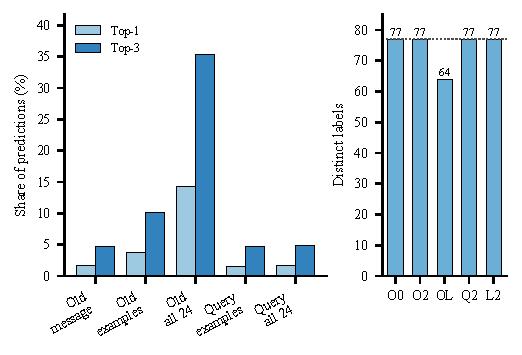
\includegraphics[width=\linewidth]{fig_concentration.pdf}
\caption{Prediction concentration from the stored per-row predictions. Left:
share of rows assigned to the single most frequent label (top-1) and to the
three most frequent labels (top-3). Right: number of distinct labels used out
of \PLabels{}. The old head at \PSeq{} bytes collapses onto a subset of labels;
the query head restores the full label range. O0, O2, OL, Q2 and L2 are the
old message-only, old examples, old all-24, query examples and \PSeq-byte query
all-24 arms.}
\label{fig:concentration}
\end{figure}

\subsection{The fix does not close the gap}

The query head with examples is \PQueryTwoAcc\%, which is \PQueryGapAbs{} points
below Jev. It is also only \PQueryVsOldZero{} points above the old head's
message-only arm, and that difference is not significant
(\PQueryVsOldZeroPText; bootstrap lower \PQueryVsOldZeroLower). The point
estimate is higher, but the data do not distinguish it from a head that reads
only the message. At this budget the retrieved examples recover what mean
pooling destroyed and buy almost nothing beyond the message itself.

The no-example query arm is \PQueryZeroAcc\%, but it is out of distribution:
the query head was trained only on contexts containing examples. It is a
control for the example context, not a fair no-example baseline. With that
caveat, the \PSeq-byte head clearly learned to use the examples---it is
\PLenVsLenZero{} points above its own message-only control---but the net effect
against the message-only old head is still negative.

\subsection{All the examples fit, and accuracy falls}

The \PSeq-byte arm removes the native-window example constraint. All
\PExamples{} examples fit (mean \PLenEff, range \PLenEffMin--\PLenEffMax), the
mean context is \PLenTwoContext{} bytes, and the head is trained jointly at the
longer length for \PSteps{} steps. It reaches \PLenTwoAcc\% (95\% Wilson
\PLenTwoLo--\PLenTwoHi), \PLenTwoGap{} points below Jev. Against the
native-window query head it loses \PLenVsNative{} points (exact McNemar
\PLenVsNativePText; bootstrap lower \PLenVsNativeLower); against the old
message-only head it loses \PLenVsOldZero{} points (\PLenVsOldZeroPText;
bootstrap lower \PLenVsOldZeroLower). It does beat the old head on the same
packed contexts by \PLenMechGain{} points, so the query pool is still doing its
job. The problem is that the longer, example-rich context is not a better
decision context for this schedule.

The training/test separation bounds the claim. On the \PTrainN{} training rows
the final head reaches \PTrainAcc\% (\PTrainCorrect/\PTrainN) with a mean
cross-entropy of \PTrainLoss; the test accuracy is \PTestAcc\%. The
test-minus-train gap is \PTrainGap{} points, the direction expected when
capacity is large relative to the training set \citep{zhang2017rethinking}. No
early stopping or checkpoint selection was used, so this is the separation of
the step-\PSteps{} head, not a selected best case. A head that fits
\PTrainAcc\% of its training rows and still misses the bar is evidence about
what it can extract from the context, not evidence that a longer fine-tune
would close the gap.

\subsection{Where the rows move}

Table~\ref{tab:transitions} replaces the aggregate accuracy with the row-level
movement behind it. The query head with examples wins more rows than it loses
against the old message-only head, but the net is small and the paired test is
not significant (\PQueryVsOldZeroPText). Against the old head on the same
contexts it wins most of the discordant rows, so the pooling recovery is broad
rather than a few rescued outliers. The \PSeq-byte arm loses more rows than it
wins against both the native query head and the old message-only head. Moving
to the longer context is not a wash: the losses are concentrated in the
example-rich conditions, exactly where the longer window was supposed to help.

\begin{table*}[t]
\centering
\footnotesize
\caption{Exact McNemar transition counts between selected arms. ``Wins'' are
rows the left arm gets right and the right arm gets wrong; ``losses'' are the
reverse. Positive net means the left arm is correct on more rows. $\Delta$ is
the accuracy difference in points. Every count is recomputed from the stored
per-row vectors; the table is generated with
\texttt{paper/gen\_paper.py}.}
\label{tab:transitions}
\setlength{\tabcolsep}{3pt}
\begin{tabular}{@{}lrrrrr@{}}
\toprule
Comparison & Wins & Losses & Net & $\Delta$ (pp) & McNemar $p$ \\
\midrule
Query ex. vs old msg. & 152 & 132 & +20 & +0.65 & $2.60\times10^{-1}$ \\
Query ex. vs old ex. & 986 & 65 & +921 & +29.90 & $3.62\times10^{-212}$ \\
Long all 24 vs query ex. & 81 & 140 & -59 & $-1.92$ & $8.75\times10^{-5}$ \\
Long all 24 vs old msg. & 149 & 188 & -39 & $-1.27$ & $3.83\times10^{-2}$ \\
Old ex. vs old msg. & 99 & 1{,}000 & -901 & $-29.25$ & $4.23\times10^{-188}$ \\
Long all 24 vs long msg. & 847 & 66 & +781 & +25.36 & $1.27\times10^{-173}$ \\
\bottomrule
\end{tabular}
\end{table*}


\subsection{The example budget is not the explanation}

The natural hypothesis after the native-window result is that the model simply
did not have room for the examples: \PNativeBudget{} bytes hold only
\PQueryEff{} of \PExamples{}, on average. The \PSeq-byte arm tests that
hypothesis and rejects it as a complete explanation. All \PExamples{} examples
fit, and accuracy is lower than the native-window query head and lower than the
message-only old head. More examples, in this schedule, are negative transfer.

Two things remain confounded, and we state them rather than choosing one. The
\PSeq-byte arm is a joint fine-tune, so length and head training move together;
it cannot separate ``the encoder was trained at \PSeq{} bytes'' from ``the head
was trained on longer contexts''. And the arm still lacks the \PLabels{}
category definitions. The reconstructed comparator prompt is
\PJevPromptMedian{} bytes in the median; the definitions are \PJevDefsBytes{} of
those bytes, and the retrieved examples are \PJevExamplesMedian{} bytes. Our
largest context is \PAzuriteShare\% of the median prompt. Even if every example
is present, the information budget is not matched. The comparison can reject
the examples-only explanation; it cannot attribute the remaining gap to
architecture alone.

This is the information-budget bound the experiment supports. Adding examples
from \PQueryEff{} to \PExamples{} does not add accuracy; the largest context
effect we measure is \PQueryVsOldZero{} points, while the gap to Jev is
\PLenTwoGapAbs{} points. A definitions-only intervention at \PSeq{} bytes would
need to recover several times the largest context effect measured here, and it
would still be a different information budget from the comparator's
\PJevPromptMedian-byte prompt. That intervention is the next pre-registered
question, not a result of this paper.

\section{Discussion}

\paragraph{Constraint is not accuracy.}
A decider's guarantee is that the answer is in the candidate set. That
guarantee is real and worth having, but it says nothing about whether the
selected candidate is correct. Our result makes the distinction concrete: the
best arm never emits an out-of-bank label and still misses \PQueryGapAbs{}
points of accuracy. Reports that quote only the constraint, or only a
single-draw accuracy, do not support the comparative claim.

\paragraph{Retrieval is not free.}
Adding retrieved examples is usually treated as adding information. For a
mean-pooled encoder it also adds noise to the representation: the message
becomes a small fraction of the pooled vector. The head control shows that this
is not a data problem---the query head reads the same contexts and recovers
\PMechGain{} points---but it is also not a complete fix, because the recovered
accuracy is still only the message-only accuracy. Retrieval should be evaluated
as a change to the read-out, not only as a change to the input.

\paragraph{Context length can be negative transfer.}
The \PSeq-byte arm is the clearest negative result in the paper. All examples
fit, the head is trained at the longer length, and accuracy falls relative to
both the native query head and the message-only old head. Longer contexts are
not automatically better; they change the distribution of the pooled
representation and the effective position of the message. This is consistent
with the long-context literature's warning that position and retrieval quality
matter, not just window size \citep{liu2023lost,hsieh2024ruler}, though our
scale is much smaller.

\paragraph{What a decider comparison should report.}
At minimum: the exact row set; the exact examples or retrieval procedure; the
category definitions or other prompt content; the context budget in bytes or
tokens; the head and pooling operation; the training rows and whether they
overlap the test rows; the number of seeds; and paired tests against the
comparator's per-row correctness, not just two independent intervals. Our
records satisfy those requirements, and the missing definitions are stated as a
limitation rather than hidden.

\paragraph{What would change the verdict.}
Three interventions are worth distinguishing, and none of them is a repair of
the current record. A definitions-only arm at \PSeq{} bytes would test whether
the missing \PLabels{} definitions, rather than the examples or the pooling,
account for the gap; it needs its own pre-registration because it changes the
information budget. A length-only arm with a separate masked-LM adaptation
would separate length from head training, which the joint schedule in this
paper cannot do. A seed study at the same budget would tell us whether the
\PQueryVsOldZero{} point difference is stable, though the paired interval
already says it is not distinguishable from zero at this sample size. If a
definitions-only arm also misses, the honest conclusion is that this model
class and budget are short of the bar, not that another head will recover it.

\paragraph{Limitations.}
The experiment is one model size, one task, one seed and one head family per
arm; scaling is jointly determined by parameters, data and compute, and a
single rung cannot identify that surface \citep{kaplan2020scaling,hoffmann2022chinchilla}.
We do not claim a seed distribution. The old-head \PSeq-byte arm and the
query-head \PSeq-byte arm come from different evaluations with different
packing; the table marks the distinction, and the native-window comparison is
the clean one. The \PSeq-byte arm is a joint fine-tune, so length and head
training are confounded. The Jev vector is third-party; we freeze it rather
than rerun the service, and a wrong Jev bit would change the paired tests. The
prompt-budget reconstruction is a reconstruction, not a capture of the exact
vendor payload. The encoder is text-only and byte-level; nothing here tests
multimodality, and \PSeq{} bytes is not a long-context regime. Finally, the
category definitions are absent from every Azurite arm, so the comparison is
deliberately unequal in Jev's favour and cannot support a claim of architectural
superiority.

\section{Conclusion}

We ran the comparison a decider claim needs: the full official Banking77 test
set, the exact retrieved examples, the frozen Jev correctness vector, a
pre-registered decision rule, and a head change that isolates the read-out. The
best arm reaches \PQueryTwoAcc\%, \PQueryGapAbs{} points below Jev, and misses
the bar. The immediate cause is mean pooling: examples dilute the message, and
a message-query attention pool recovers \PMechGain{} points on identical
contexts. The fix is not sufficient. The query head is statistically
indistinguishable from the old head's message-only arm, and a \PSeq-byte joint
fine-tune with all \PExamples{} examples is worse than both the native query
head and the message-only head. The comparator's JSON prompt is
\PJevPromptRatio$\times$ our largest context and contains the definitions we
withhold, so the experiment bounds the claim to a smaller information budget.
The honest conclusion is not that deciders fail; it is that this decoder, at
this budget, with this read-out, does not meet the bar, and that the next lever
is information parity rather than another pooling variant.

\section*{Reproducibility}

The generator \texttt{paper/gen\_paper.py} reads
\texttt{results/jev\_query/eval/summary.json},
\texttt{results/jev\_query\_5120/eval/summary.json} and
\texttt{results/jev\_matched/summary.json}, verifies every per-example SHA-256,
recomputes every statistic, and writes \texttt{paper/generated/macros.tex},
the tables, the figures and \texttt{paper/RECONCILIATION.md}. The public prompt
inputs are vendored under \texttt{paper/data/jev\_prompt} with their own hashes
and source record. Rebuilding is
\texttt{python paper/gen\_paper.py \&\& cd paper \&\& tectonic azurite.tex}.

\bibliography{refs}

\appendix

\section{Statistical definitions}

For an arm with $k$ correct rows out of $n$, the 95\% Wilson interval is
\begin{equation}
\frac{\hat p+\frac{z^2}{2n}\pm z\sqrt{\frac{\hat p(1-\hat p)}{n}+\frac{z^2}{4n^2}}}{1+\frac{z^2}{n}},
\end{equation}
with $z=1.959963984540054$ and $\hat p=k/n$ \citep{wilson1927}. For two aligned
correctness vectors, the exact McNemar test counts the discordant pairs
$b$ (left correct, right wrong) and $c$ (left wrong, right correct) and reports
the two-sided binomial tail at $p=1/2$ \citep{mcnemar1947}. The paired bootstrap
resamples rows with replacement, computes the mean difference in each of
\PBOOT{} draws and reports the 5th percentile; the seed is 0. The P0 rule and
the non-inferiority margin are fixed in \S\ref{sec:decision}. All three quantities are
recomputed from the stored per-row vectors by \texttt{paper/gen\_paper.py}.

\section{Content identities and reproduction}

\begin{table}[t]
\centering
\footnotesize
\caption{Content identities for the records the paper reads. Each is the first
12 hex digits of a SHA-256; the full values and the per-example hashes are in
the stored summaries and \texttt{paper/RECONCILIATION.md}.}
\label{tab:hashes}
\begin{tabular}{@{}ll@{}}
\toprule
Artifact & SHA-256 (first 12) \\
\midrule
Query pre-registration & \texttt{bde97e74f2f8} \\
Query inputs & \texttt{8dccd8c89886} \\
Query code & \texttt{95a5e0a5d11e} \\
Old head & \texttt{42f1ed1c8471} \\
Query head & \texttt{7992c97362b3} \\
5,120 pre-registration & \texttt{c59b5e08d916} \\
5,120 amendment & \texttt{7993177d769a} \\
5,120 init checkpoint & \texttt{5294fd685615} \\
5,120 head & \texttt{e7455fc462e9} \\
5,120 code & \texttt{0800b2aad102} \\
\bottomrule
\end{tabular}
\end{table}


The full SHA-256 values and per-example hashes are in
\texttt{paper/RECONCILIATION.md} and the three summary JSON files. The
reconciliation step also checks the shared values against the thesis macros, so
the paper and the thesis cannot drift apart silently.

\paragraph{Records.}
The query evaluation is under \texttt{results/jev\_query/}; the \PSeq-byte
evaluation under \texttt{results/jev\_query\_5120/}; the matched-test and the
old-head \PSeq-byte arm under \texttt{results/jev\_matched/}. 

\end{document}
